%----------------------------------------------------------------------------
% Magic tutorial number 2
%----------------------------------------------------------------------------

\NeedsTeXFormat{LaTeX2e}[1994/12/01]
\documentclass[letterpaper,twoside,12pt]{article}
\usepackage{epsfig,times}

\setlength{\textwidth}{8.5in}
\addtolength{\textwidth}{-2.0in}
\setlength{\textheight}{11.0in}
\addtolength{\textheight}{-2.0in}
\setlength{\oddsidemargin}{0in}
\setlength{\evensidemargin}{0pt}
\setlength{\topmargin}{-0.5in}
\setlength{\headheight}{0.2in}
\setlength{\headsep}{0.3in}
\setlength{\topskip}{0pt}

\def\hinch{\hspace*{0.5in}}
\def\starti{\begin{center}\begin{tabbing}\hinch\=\hinch\=\hinch\=hinch\=\kill}
\def\endi{\end{tabbing}\end{center}}
\def\ii{\>\>\>}
\def\mytitle{Magic Tutorial \#2: Basic Painting and Selection}

%----------------------------------------------------------------------------

\begin{document}

\makeatletter
\newcommand{\ps@magic}{%
	\renewcommand{\@oddhead}{\mytitle\hfil\today}%
	\renewcommand{\@evenhead}{\today\hfil\mytitle}%
	\renewcommand{\@evenfoot}{\hfil\textrm{--{\thepage}--}\hfil}%
	\renewcommand{\@oddfoot}{\@evenfoot}}
\newcommand{\ps@mplain}{%
	\renewcommand{\@oddhead}{}%
	\renewcommand{\@evenhead}{}%
	\renewcommand{\@evenfoot}{\hfil\textrm{--{\thepage}--}\hfil}%
	\renewcommand{\@oddfoot}{\@evenfoot}}
\makeatother
\pagestyle{magic}
\thispagestyle{mplain}


\begin{center}
  {\bfseries \Large \mytitle} \\
  \vspace*{0.5in}
  {\itshape John Ousterhout} \\
  \vspace*{0.5in}
   Computer Science Division \\
   Electrical Engineering and Computer Sciences \\
   University of California \\
   Berkeley, CA  94720 \\
  \vspace*{0.25in}
  {\itshape (Updated by others, too.)} \\
  \vspace*{0.25in}
  This tutorial corresponds to Magic version 7. \\
\end{center}
\vspace*{0.5in}

{\noindent\bfseries\large Tutorials to read first:}
\starti
   \> Magic Tutorial  \#1: Getting Started
\endi

{\noindent\bfseries\large Commands introduced in this tutorial:}
\starti
   \> :box, :clockwise, :copy, :erase, :findbox :grid, :label, \\
   \> :layers, :macro, :move, :paint, :redo, :save, :select, \\
   \>:sideways, :undo, :upsidedown, :view, :what, :writeall, :zoom
\endi

{\noindent\bfseries\large Macros introduced in this tutorial:}

\starti
   \> a, A, c, d, \^{}D, e, E, g, G, q, Q, r, R, s, S, t, T, u, U, v, w, W, z, Z, 4
\endi

\vspace*{0.75in}
\section{Cells and Paint}

In Magic, a circuit layout is a hierarchical collection
of {\itshape cells}.  Each cell contains three things:
colored shapes, called {\itshape paint}, that define the circuit's structure;
textual {\itshape labels} attached to the paint;  and
{\itshape subcells}, which are instances of other cells.  The paint
is what determines the eventual function of the VLSI circuit.  Labels
and subcells are a convenience for you in managing
the layout and provide a way of communicating information
between various synthesis and analysis tools.  This tutorial
explains how to create and edit paint and labels in simple
single-cell designs, using the basic painting commands.
``Magic Tutorial  \#3: Advanced Painting (Wiring and Plowing)''
describes some more advanced features for manipulating paint.
For information on how to build up cell
hierarchies, see ``Magic Tutorial  \#4:  Cell Hierarchies''.

\section{Painting and Erasing}

Enter Magic to edit the cell {\bfseries tut2a} (type {\bfseries magic tut2a}
to the Unix shell;  follow the directions in ``Tutorial \#1: Getting
Started'' if you have any problems with this).  The {\bfseries tut2a}
cell is a sort of palette:  it shows a splotch of each of several
paint layers and gives the names that Magic uses for the layers.

The two basic layout operations are painting and erasing.  They
can be invoked using the {\bfseries :paint} and {\bfseries :erase}
long commands, or using the buttons.  The easiest way to paint
and erase is with the mouse buttons.  To paint, 
position the box over the area
you'd like to paint, then move the cursor over a color
and click the middle mouse button.  To erase
everything in an area, place the box over the area, move the
cursor over a blank spot, and click the middle mouse button.
Try painting and erasing various colors.  If the screen gets
totally messed up, you can always exit Magic and restart it.
While you're painting, white dots may occasionally appear
and disappear.  These are design rule violations detected
by Magic, and will be explained in ``Magic Tutorial \#6: Design
Rule Checking''.  You can ignore them for now.

It's completely legal to paint one layer on top of another.
When this happens, one of three things may occur.  In some
cases, the layers are independent, so what you'll see is
a combination of the two, as if each were a transparent colored
foil.  This happens, for example, if you paint metal1 (blue) on
top of polysilicon (red).  In other cases, when you paint one
layer on top of another you'll get something different from
either of the two original layers.  For example, painting
poly on top of ndiff produces ntransistor (try
this).  In still other cases the
new layer replaces the old one:  this happens, for example,
if you paint a pcontact on top of ntransistor.
Try painting different layers on top of each other to see
what happens.  The meaning of the various layers is discussed
in more detail in Section 11 below.

There is a second way of erasing paint that allows you to
erase some layers without affecting others.  This is the
macro {\bfseries \^{}D} (control-D, for ``{\bfseries D}elete paint'').  To use it,
position the box over the area to be erased, then move
the crosshair over a splotch of paint containing the
layer(s) you'd like to erase.  Type {\bfseries \^{}D} key on
the text keyboard: the colors underneath the cursor will
be erased from the area underneath the box, but no other
layers will be affected.  Experiment around with the {\bfseries \^{}D}
macro to try different combinations of paints and erases.
If the cursor is over empty space then the {\bfseries \^{}D}
macro is equivalent to the middle mouse button:  it erases
everything.

You can also paint and erase using the long commands

\starti
   \ii {\bfseries :paint} {\itshape layers} \\
   \ii {\bfseries :erase} {\itshape layers}
\endi

In each of these commands {\itshape layers} is one or more layer
names separated by commas (you can also use spaces for separators,
but only if you enclose the entire list in double-quotes).  Any
layer can be abbreviated as long as the abbreviation is
unambiguous.  For example, {\bfseries :paint poly,metal1} will
paint the polysilicon and metal1 layers.  The macro {\bfseries \^{}D}
is predefined by Magic to be {\bfseries :erase \$} ({\bfseries \$} is a
pseudo-layer that means ``all layers underneath the cursor'').

\section{Undo}

There are probably going to be times when you'll do things that
you'll later wish you hadn't.  Fortunately, Magic has an
undo facility that you can use to restore things after you've
made mistakes.  The command

\starti
   \ii {\bfseries :undo}
\endi

(or, alternatively, the macro {\bfseries u}) will undo the effects of
the last command you invoked.
If you made a mistake several commands back, you can type
{\bfseries :undo} several times to undo successive commands.
However, there is a limit to all this:  Magic only remembers
how to undo the last ten or so commands.  If you
undo something and then decide you wanted it after all, you
can undo the undo with the command

\starti
   \ii {\bfseries :redo}
\endi

({\bfseries U} is a macro for this command).  Try making a few paints
and erases, then use {\bfseries :undo} and {\bfseries :redo} to work
backwards and forwards through the changes you made.

\section{The Selection}

Once you have painted a piece of layout, there are several commands
you can invoke to modify the layout.  Many of them are based on
the {\itshape selection}:  you select one or more pieces of the design,
and then perform operations such as copying, deletion, and rotation
on the selected things.
To see how the selection works, load cell {\bfseries tut2b}.  You
can do this by typing {\bfseries :load tut2b} if you're still in Magic,
or by starting up Magic with the shell command {\bfseries magic tut2b}.

The first thing to do is to learn how to select.
Move the cursor over the upper portion of the
L-shaped blue area in {\bfseries tut2b}, and type {\bfseries s}, which
is a macro for {\bfseries :select}.  The box
will jump over to cover the vertical part of the ``L''.  This
operation selected a chunk of material.  Move the box away from
the chunk, and you'll see that a thin white outline is left
around the chunk to show that it's selected.  Now move the cursor
over the vertical red bar on the right of the cell and type {\bfseries s}.
The box will move over that bar, and the selection highlighting will
disappear from the blue area.

If you type {\bfseries s} several times without moving the cursor,
each command selects a slightly larger piece of material.  Move the
cursor back over the top of the blue ``L'', and type {\bfseries s} three
times without moving the cursor.  The first {\bfseries s} selects a
chunk (a rectangular region all of the same type of material).  The
second {\bfseries s} selects a {\itshape region} (all of the
blue material in the region underneath the cursor, rectangular or not).
The third {\bfseries s} selects a {\itshape net} (all of the material that is
electrically connected to the original chunk; this includes the
blue metal, the red polysilicon, and the contact that connects them).

The macro {\bfseries S} (short for {\bfseries :select more}) is just like {\bfseries s}
except that it adds on to the selection, rather than replacing it.
Move the cursor over the vertical red bar on the right
and type {\bfseries S} to see how this works.  You can also type {\bfseries S}
multiple times to add regions and nets to the selection.

If you accidentally type {\bfseries s} or {\bfseries S} when the cursor is
over space, you'll select a cell ({\bfseries tut2b} in this case).
You can just undo this for now.  Cell selection will be discussed
in ``Magic Tutorial \#4: Cell Hierarchies''.

You can also select material by area:  place the box
around the material you'd like to select and type {\bfseries a} (short
for {\bfseries :select area}).  This will select all of the material
underneath the box.
You can use the macro {\bfseries A} to add material to the selection
by area, and you can use the long command

\starti
   \ii {\bfseries :select }[{\bfseries more}]{\bfseries  area} {\itshape layers}
\endi

to select only material on certain layers.  Place the box around
everything in {\bfseries tut2b} and type {\bfseries :select area metal1}
followed by {\bfseries :select more area poly}.

If you'd like to clear out the selection without modifying any
of the selected material, you can use the command

\starti
   \ii {\bfseries :select clear}
\endi

or type the macro {\bfseries C}.  You can clear out just a portion of
the selection by typing {\bfseries :select less} or {\bfseries :select less
area} {\itshape layers}; the former deselects paint in the order that
{\bfseries :select} selects paint, while the latter deselects
paint under the box (just as {\bfseries :select area} selects paint
under the box).
For a synopsis of all the options
to the {\bfseries :select} command, type

\starti
   \ii {\bfseries :select help}
\endi


\section{Operations on the Selection}

Once you've made a selection, there are a number of operations you
can perform on it:

\starti
   \ii {\bfseries :delete} \\
   \ii {\bfseries :move }[{\itshape direction} [{\itshape distance}]] \\
   \ii {\bfseries :stretch }[{\itshape direction} [{\itshape distance}]] \\
   \ii {\bfseries :copy} \\
   \ii {\bfseries :upsidedown} \\
   \ii {\bfseries :sideways} \\
   \ii {\bfseries :clockwise }[{\itshape degrees}] \\
\endi

The {\bfseries :delete} command deletes everything that's selected.
Watch out:  {\bfseries :delete} is different from {\bfseries :erase}, which erases
paint from the area underneath the box.
Select the red bar on the right in {\bfseries tut2b} and type {\bfseries d},
which is a macro for {\bfseries :delete}.  Undo the deletion with the
{\bfseries u} macro.

The {\bfseries :move} command picks up both the box
and the selection and moves them so that the lower-left corner of
the box is at the cursor location.  Select the red bar on the right
and move it so that it falls on top of the vertical part of
the blue ``L''.  You can use {\bfseries t} (``{\bfseries t}ranslate'') as a macro
for {\bfseries :move}.  Practice moving various things around the screen.
The command {\bfseries :copy} and its macro {\bfseries c} are just like
{\bfseries :move} except that a copy of the selection is left behind at
the original position.

There is also a longer form of the {\bfseries :move} command that you
can use to move the selection a precise amount.  For example,
{\bfseries :move up 10} will move the selection (and the box) up
10 units.  The
{\itshape direction} argument can be any direction like {\bfseries left},
{\bfseries south}, {\bfseries down}, etc.  See the Magic manual page for
a complete list of the legal directions.   The macros {\bfseries q},
{\bfseries w}, {\bfseries e}, and {\bfseries r} are defined to move the selection
left, down, up, and right (respectively) by one unit.

The {\bfseries :stretch} command is similar to {\bfseries :move} except that
it stretches and erases as it moves.  {\bfseries :stretch}  does not
operate diagonally, so if you use the cursor to indicate where
to stretch to, Magic will either stretch up, down, left, or right,
whichever is closest.  The {\bfseries :stretch} command moves the selection
and also does two additional things.  First, for each piece of paint
that moves, {\bfseries :stretch} will erase that layer from the region that
the paint passes through as it moves, in order to clear material out
of its way.  Second, if the back edge of a piece of selected paint touches
non-selected material, one of the two pieces of paint is stretched to
maintain the connection.  The macros {\bfseries Q}, {\bfseries W}, {\bfseries E}, and {\bfseries R}
just like
the macros {\bfseries q}, etc. described above for {\bfseries :move}.  The macro
{\bfseries T} is predefined to {\bfseries :stretch}.
To see how stretching works, select the horizontal
piece of the green wire in {\bfseries tut2b} and type {\bfseries W}, then {\bfseries E}.
Stretching only worries about material in front of and behind the
selection;  it ignores material to the sides (try the {\bfseries Q} and {\bfseries R}
macros to see).  You can use plowing (described in Tutorial  \#3) if this is a
problem.

The command {\bfseries :upsidedown} will flip the selection upside
down, and {\bfseries :sideways} flips the selection sideways.  Both
commands leave the selection so it occupies the same total area
as before, but with the contents flipped.  The command
{\bfseries :clockwise} will rotate the selection clockwise, leaving the
lower-left corner of the new selection at the same place as the
lower-left corner of the old selection.  {\itshape Degrees}
must be a multiple of 90, and defaults to 90.

At this point you know enough to do quite a bit of damage
to the {\bfseries tut2b} cell.  Experiment with the selection
commands.  Remember that you can use {\bfseries :undo} to back
out of trouble.

\section{Labels}

Labels are pieces of text attached to the paint of a cell.
They are used to provide information to other tools that will
process the circuit.  Most labels are node names: they provide
an easy way of referring to nodes in tools such as routers, simulators,
and timing analyzers.  Labels may also be used for other purposes:
for example, some labels are treated as {\itshape attributes} that
give Crystal, the timing analyzer, information about the
direction of signal flow through transistors.

Load the cell {\bfseries tut2c} and place a cross in the middle of
the red chunk (to make a cross, position the lower-left corner
of the box with the left button and then click the right button
to place the upper-right corner on top of the lower-left corner).
Then type
type the command {\bfseries :label test}.  A new label will appear
at the position of the box.  The complete syntax of the {\bfseries :label}
command is

\starti
   \ii {\bfseries :label }[{\itshape text }[{\itshape position }[{\itshape layer}]]]
\endi

{\itshape Text} must be supplied, but the other arguments can be
defaulted.  If {\itshape text} has any spaces in it, then it must
be enclosed in double quotes.  {\itshape Position} tells where
the text should be displayed, relative to the point of the
label.  It may be any of {\bfseries north}, {\bfseries south}, {\bfseries east},
{\bfseries west}, {\bfseries top}, {\bfseries bottom}, {\bfseries left},
{\bfseries right}, {\bfseries up}, {\bfseries down}, {\bfseries center},
{\bfseries northeast}, {\bfseries ne}, {\bfseries southeast}, {\bfseries se},
{\bfseries southwest}, {\bfseries sw}, {\bfseries northwest}, {\bfseries nw}.
For example, if {\bfseries ne} is given, the text will be displayed above and
to the right of the label point.  If no {\itshape position} is given,
Magic will pick a position for you.  {\itshape Layer} tells which paint
layer to attach the label to.  If {\itshape layer} covers the entire
area of the label, then the label will be associated with the
particular layer.  If {\itshape layer} is omitted, or if it doesn't
cover the label's area, Magic initially associates the label with
the ``space'' layer, then checks to see if there's a layer that covers the
whole area.  If there is, Magic moves the label to that layer.
It is generally a bad idea to place labels
at points where there are several paint layers, since it will
be hard to tell which layer the label is attached to.
As you edit, Magic will ensure that labels are only
attached to layers that exist everywhere under the label.
To see how this works,
paint the layer pdiff (brown) over the label you just
created:  the label will
switch layers.  Finally, erase poly over the area, and
the label will move again.

Although many labels are point labels, this need not be the case.
You can label any rectangular area by setting the box to that
area before invoking the label command.  This feature is used for
labelling terminals for the router (see below), and for labelling tiles used
by Mpack, the tile packing program.  {\bfseries Tut2c} has examples of
point, line, and rectangular labels.

All of the selection commands apply to labels as well as paint.
Whenever you select paint, the labels attached to that paint
will also be selected.  Selected labels are highlighted in white.
Select some of the chunks of paint in {\bfseries tut2c}
to see how the labels are selected too.  When you use
area selection, labels will only be selected if they are completely
contained in the area being selected.  If you'd like to select
{\itshape just} a label without any paint, make the box into a cross
and put the cross on the label:  {\bfseries s} and {\bfseries S} will select
just the label.

There are several ways to erase a label.  One way is to select and then
delete it.  Another way is to erase the paint that the label is attached
to.  If the paint is erased all around the label, then Magic will delete
the label too.  Try attaching a
label to a red area, then paint blue over the red.
If you erase blue the label stays (since it's attached
to red), but if you erase the red then the label is deleted.

You can also erase labels using the {\bfseries :erase} command
and the pseudo-layer {\bfseries labels}.  The command

\starti
   \ii {\bfseries :erase labels}
\endi

will erase all labels that lie completely within the area of the box.
Finally, you can erase a label by making
the box into a cross on top of the label, then clicking the middle
button with the cursor over empty space.  Technically, this will
erase all paint layers and labels too.  However, since the
box has zero area, erasing paint has no effect:  only the labels
are erased.

\section{Labelling Conventions}

When creating labels, Magic will permit you
to use absolutely any text whatsoever.  However, many
other tools, and even parts of Magic, expect label names
to observe certain conventions.  Except for the special cases
described below, labels shouldn't contain any of the characters
``/\$@!\^{}''.  Spaces, control characters, or parentheses
within labels are probably a bad idea too.
Many of the programs that process Magic output
have their own restrictions on label names, so you should
find out about the restrictions that apply at your site.
Most labels are node
names: each one gives a unique identification to a set of things that
are electrically connected.  There are two kinds of node
names, local and global.  Any label that ends in ``!''
is treated as a global node name;  it will be assumed
that all nodes by this name, anywere in any cell in a layout, are
electrically connected.  The most common global names are
{\bfseries Vdd!} and {\bfseries GND!}, the power rails.  You should
always use these names exactly, since many other tools
require them.  Nobody knows why ``GND!'' is all in capital letters
and ``Vdd!'' isn't.

Any label that does not end in ``!'' or any of the other
special characters discussed below is a local node name.
It refers to a node within that particular cell.  Local
node names should be unique within the cell: there shouldn't
be two electrically distinct nodes with the same name.
On the other hand, it is perfectly legal, and sometimes
advantageous, to give more than one name to the same node.
It is also legal to use the same local node name in different
cells:  the tools will be able to distinguish between them
and will not assume that they are electrically connected.

The only other labels currently understood by the tools
are {\itshape attributes}.  Attributes are pieces of text associated
with a particular piece of the circuit:  they are not node
names, and need not be unique.  For example, an attribute
might identify a node as a chip input, or it might identify
a transistor terminal
as the source of information for that transistor.  Any label
whose last character is ``@'', ``\$'', or ``\^{}''  is an attribute.  There
are three different kinds of attributes.  Node attributes are
those ending with ``@'';  they are associated with particular
nodes.  Transistor source/drain attributes are those ending in ``\$'';
they are associated with particular terminals of a transistor.
A source or drain attribute must be attached to the channel region
of the transistor and must fall exactly on the source or drain
edge of the transistor.  The third kind of attribute is a
transistor gate attribute.  It ends in ``\^{}'' and is attached to
the channel region of the transistor.
To see examples of attributes and node names, edit the cell
{\bfseries tut2d} in Magic.

Special conventions apply to labels for routing terminals.  The standard
Magic router (invoked by {\bfseries :route})
ignores all labels except for those on the edges of cells.  (This restriction
does not apply to the gate-array router, Garoute, or to the interactive
router, Iroute).  If you expect to use the 
standard router to connect to a particular node,
you should place the label for that node on its outermost edge.
The label should not be a point label, but should instead be
a horizontal or vertical line covering the entire edge of the
wire.  The router will choose a connection point somewhere
along the label.
A good rule of thumb is to label all nodes that enter or leave
the cell in this way.  For more details on how labels are used
by the standard router, see ``Magic Tutorial  \#7:  Netlists and Routing''.  
Other labeling conventions are used by the Garouter and Irouter, consult
their respective tutorials for details.

\section{Files and Formats}

Magic provides a variety of ways to save your cells on
disk.  Normally, things are saved in a special
Magic format.  Each
cell is a separate file, and the name of the file is
just the name of the cell with {\bfseries .mag} appended.  For
example, the cell {\bfseries tut2a} is saved in file
{\bfseries tut2a.mag}.  To save cells on disk, invoke the
command

\starti
   \ii {\bfseries :writeall}
\endi

This command will run through each of the cells that you have
modified in this editing session, and ask you what to do with
the cell.  Normally, you'll type {\bfseries write}, or just hit the
return key, in which case the cell will be written back
to the disk file from which it was read (if this is a new cell,
then you'll be asked for a name for the cell).  If you type
{\bfseries autowrite}, then Magic will write out all the cells that have
changed without asking you what to do on a cell-by-cell basis.
{\bfseries Flush} will cause Magic to delete its internal copy of the cell
and reload the cell from the disk copy, thereby expunging all edits
that you've made.  {\bfseries Skip} will pass on to the next cell without
writing this cell (but Magic still remembers that it has
changed, so the next time you invoke {\bfseries :writeall} Magic
will ask about this cell again).  {\bfseries Abort} will stop
the command immediately without writing or checking any more cells.

{\bfseries IMPORTANT NOTE:}  Unlike vi and other text editors, Magic
doesn't keep checkpoint files.  This means that if the system
should crash in the middle of a session, you'll lose all changes
since the last time you wrote out cells.  It's a good idea to
save your cells frequently during long editing sessions.

You can also save the cell you're currently editing with the command

\starti
  \ii {\bfseries :save} {\itshape name}
\endi

This command will append ``.mag'' to {\itshape name} and save the cell you
are editing in that location.  If you don't provide a
name, Magic will use the cell's name (plus the ``.mag''
extension) as the file name, and it will prompt you for
a name if the cell hasn't yet been named.

Once a cell has been saved on disk you can edit it by
invoking Magic with the command

\starti
   \ii {\bfseries magic} {\itshape name}
\endi

where {\itshape name} is the same name you used to save the
cell (no ``.mag'' extension).

Magic can also read and write files in CIF and Calma Stream formats.
See ``Magic Tutorial  \#9: Format Conversion for CIF and Calma''
for details.

\section{Plotting}

Magic can generate hardcopy plots of layouts in four ways: postscript
(color), versatec (black-and-white or color), gremlin, and pixels
(a generalized pixel-file that can be massaged in many ways).
To plot part of your design in PostScript, place the box around the
part you'd like to plot and type

\starti
   \ii {\bfseries :plot postscript}
\endi

This will generate a plot of the area of the box.  Everything
visible underneath the box will appear in more-or-less the same way
in the plot.  {\itshape Width} specifies how wide the plot will be, in
inches.  Magic will scale the plot so that the area of the box comes
out this wide.  The default for {\itshape width} is the width of the
plotter (if {\itshape width} is larger than the plotter width, it's
reduced to the plotter width).  If {\itshape layers} is given, it
specifies exactly what information is to be plotted.  Only those
layers will appear in the plot.  The special ``layer'' {\bfseries labels}
will enable label plotting.

The second form is for driving printers like color Versatecs.
It  is enabled by setting the {\itshape color} plot parameter to
{\itshape true}.  A table of stipples for the primary colors (black, cyan,
magenta abd yellow) is given in the technology file.  When the
{\itshape plot} command is given, four rasters (one for each of the colors)
are generated, separated with the proper control sequences for the printer.
Otherwise, operation is exactly as for the black-and-white case.

The third form of plotting is for generating Gremlin-format files,
which can then be edited with the Gremlin drawing system or
included in documents processed by Grn and Ditroff.  The command
to get Gremlin files is

\starti
   \ii {\bfseries :plot gremlin} {\itshape file }[{\itshape layers}]
\endi

It will generate a Gremlin-format file in {\itshape file} that describes
everything underneath the box.  If {\itshape layers} is specified, it
indicates which layers are to appear in the file;  otherwise everything
visible on the screen is output.  The Gremlin file is output without
any particular scale;  use the {\bfseries width} or {\bfseries height} commands
in Grn to scale the plot when it's printed.  You should use the {\bfseries mg}
stipples when printing Magic Gremlin plots;  these will produce the
same stipple patterns as {\bfseries :plot versatec}.

Finally, the ``pixels'' style of plotting generates a file of pixel
values for the region to be plotted.  This can be useful for input to
other image tools, or for generation of slides and viewgraphs for
presentations.  The file consists of a sequence of bytes, three for
each pixel, written from left to right and top to bottom.  Each three
bytes represent the red, green and blue values used to display the
pixel.  Thus, if the upper-left-most pixel were to be red, the first
three bytes of the file would have values of 255, 0 and 0.

The resolution of the generated file is normally 512, but can be
controlled by setting the plot parameter {\itshape pixWidth}.  It must be a
multiple of 8; Magic will round up if an inappropriate value is
entered.
The height
of the file is determined by the shape of the box.  In any case, the
actual resolution of the file is appended to the file name.  For
example, plotting a square region,  2048 pixels across, will result in
a file named something like ``magicPlot1234a-2048-2048''.

There are several plotting parameters used internally to Magic, such
as the width of the Versatec printer and the number of dots per inch
on the Versatec printer.  You can modify most of these to work with
different printers.  For details, read about the various {\bfseries :plot}
command options in the {\itshape man} page.

\section{Utility Commands}

There are several additional commands that you will probably find useful
once you start working on real cells.  The command

\starti
   \ii {\bfseries :grid }[{\itshape spacing}] \\
   \ii {\bfseries :grid }{\itshape xSpacing ySpacing} \\
   \ii {\bfseries :grid }{\itshape xSpacing ySpacing xOrigin yOrigin} \\
   \ii {\bfseries :grid off}
\endi

will display a grid over your layout.  Initially, the grid has
a one-unit spacing.  Typing {\bfseries :grid} with no arguments
will toggle the grid on and off.
If a single numerical argument is given, the grid
will be turned on, and the grid lines will be {\itshape spacing}
units apart.  The
macro {\bfseries g} provides a short form for {\bfseries :grid} and {\bfseries G}
is short for {\bfseries :grid 2}.  If you provide two arguments to
{\bfseries :grid}, they are the x- and y-spacings, which may be different.
If you provide four arguments, the last two specify a reference
point through which horizontal and vertical grid lines pass;  the
default is to use (0,0) as the grid origin.  The command {\bfseries :grid off}
always turns the grid off, regardless of whether or not is was
previously on.
When the grid is on, a small black box is displayed to mark the
(0,0) coordinate of the cell you're editing.

If you want to create a cell that doesn't fit on the screen,
you'll need to know how to change the screen view.  This
can be done with three commands:

\starti
   \ii {\bfseries :zoom }{\itshape factor} \\
   \ii {\bfseries :findbox }[{\bfseries zoom}] \\
   \ii {\bfseries :view}
\endi

If {\itshape factor} is given to the zoom command, 
it is a zoom-out factor.  For example,
the command {\bfseries :zoom 2} will change the view so that there are
twice as many units across the screen as there used to be ({\bfseries Z}
is a macro for this).  The
new view will have the same center as the old one.  The command
{\bfseries :zoom .5} will increase the magnification so that
only half as much of the circuit is visible.

The {\bfseries :findbox} command is used to change the view according to the box.
The command alone just moves the view (without changing the scale
factor) so that the box is in the center of the screen.  If the {\bfseries zoom}
argument is given then the magnification is changed too, so that the area of
the box nearly fills the screen.  {\bfseries z} is a macro for {\bfseries :findbox zoom}
and {\bfseries B} is a macro for {\bfseries :findbox}.

The command {\bfseries :view} resets the view so that the entire cell is visible
in the window.  It comes in handy if you get lost in a big layout.
The macro {\bfseries v} is equivalent to {\bfseries :view}.

The command {\bfseries :box} prints out the size and location of the box
in case you'd like to measure something in your layout.  The macro
{\bfseries b} is predefined to {\bfseries :box}.  The {\bfseries :box} command can also
be used to set the box to a particular location, height, or
width.  See the man page for details.

The command

\starti
   \ii {\bfseries :what}
\endi

will print out information about what's selected.  This may be helpful
if you're not sure what layer a particular piece of material is, or
what layer a particular label is attached to.

If you forget what a macro means, you can invoke the command

\starti
   \ii {\bfseries :macro }[{\itshape char}]
\endi

This command will print out the long command that's associated
with the macro {\itshape char}.  If you omit {\itshape char}, Magic will
print out all of the macro associations.  The command

\starti
  \ii {\bfseries :macro} {\itshape char command}
\endi

We set up {\itshape char} to be a macro for {\itshape command}, replacing the old
{\itshape char} macro if there was one.  If {\itshape command} contains any spaces
then it must be enclosed in double-quotes.  To see how this works, type
the command {\bfseries :macro} {\ttfamily 1 "echo You just typed the 1 key."},
then type the 1 key.

One of the macros, ``{\bfseries .}'', has special meaning in Magic.  This
macro is always defined by the system to be the last long command
you typed.  Whenever you'd like to repeat a long command, all you
have to do is use the dot macro.

\section{What the Layers Mean}

The paint layers available in Magic are different from those
that you may be used to in Caesar and other systems because
they don't correspond
exactly to the masks used in fabrication.  We call them
{\itshape abstract layers} because they correspond to constructs
such as wires and contacts, rather than mask layers.  We
also call them {\itshape logs} because they look like sticks
except that the geometry is drawn fully fleshed instead of
as lines. In Magic there
is one paint layer for each kind of conducting material
(polysilicon, ndiffusion, metal1, etc.),
plus one additional paint layer for each kind of transistor
(ntransistor, ptransistor, etc.), and, finally, one further
paint layer for each kind of contact (pcontact, ndcontact,
m2contact, etc.) Each
layer has one or more names that are
used to refer to that layer in commands.  To find out the
layers available in the current technology, type the command

\starti
   \ii {\bfseries :layers}
\endi

In addition to the mask layers, there are a few pseudo-layers
that are valid in all technologies;  these are listed in
Table~\ref{pseudolayers}.
Each Magic technology also has a technology manual describing
the features of that technology, such as design rules, routing
layers, CIF styles, etc.  If you haven't seen any of the technology
manuals yet, this is a good time to take a look at the one for
your process.

\begin{table}[hb]
   \begin{center}
      \begin{tabular}{|l|} \hline
         {\bfseries errors} (design-rule violations) \\
         {\bfseries labels} \\
         {\bfseries subcells} \\
         {\bfseries \*} (all mask layers) \\
         {\bfseries \$} (all mask layers visible under cursor) \\ \hline
      \end{tabular}
   \end{center}
   \caption{Pseudo-layers available in all technologies.}
   \label{pseudolayers}
\end{table}

If you're used to designing with mask layers (e.g. you've
been reading the Mead-Conway book), Magic's log style
will take some getting used to.
One of the reasons for logs is to
save you work.  In Magic you don't draw implants, wells, buried
windows, or contact via holes.  Instead, you draw the primary
conducting layers and paint some of their overlaps with
special types such as n-transistor or polysilicon contact.
For transistors, you draw only the
actual area of the transistor channel.  Magic will generate
the polysilicon and diffusion, plus any
necessary implants, when it creates a CIF file.  For contacts,
you paint the contact layer in the area of overlap between
the conducting layers.  Magic
will generate each of the constituent mask layers plus
vias and buried windows when it writes the CIF file. 
Figure~\ref{layers1}
shows a simple cell drawn with both mask layers (as in Caesar)
and with logs (as in Magic).  If you're curious about what
the masks will look like for a particular layout, you can use
the {\bfseries :cif see} command to view the mask information.

\begin{figure}[ht]
   \begin{center}
   \begin{minipage}{0.3\columnwidth}
      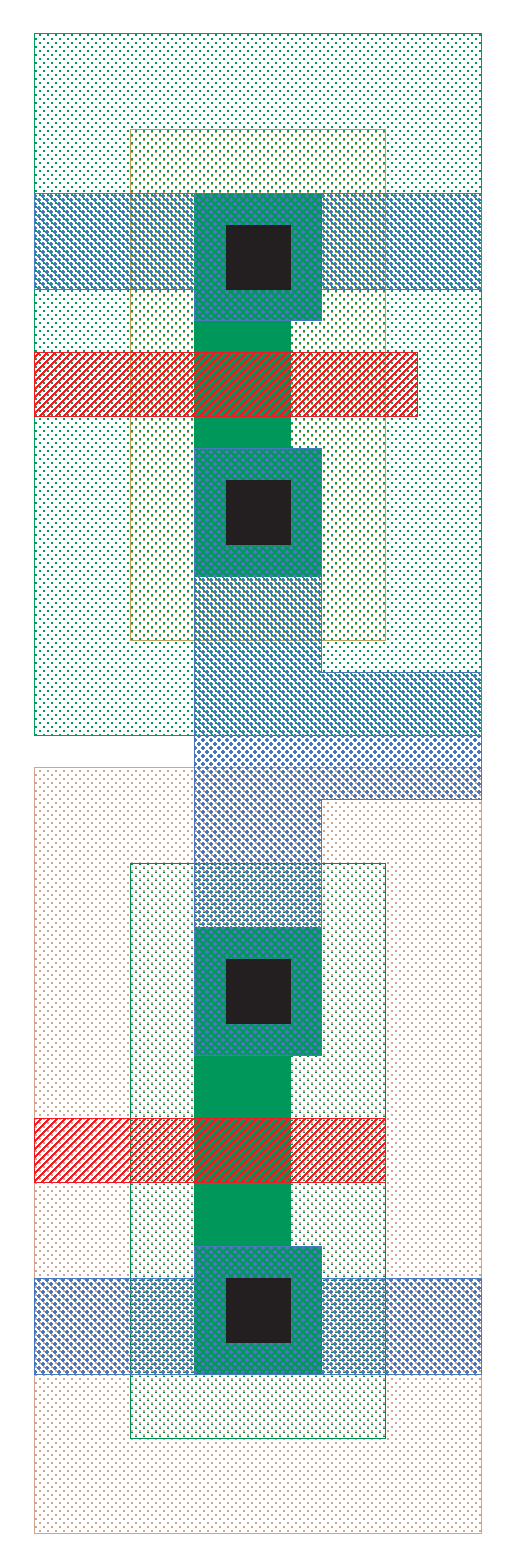
\epsfig{file=../psfigures/tut2.2.ps, height=5in}
   \end{minipage} \hspace*{0.5in}
   \begin{minipage}{0.5\columnwidth}
   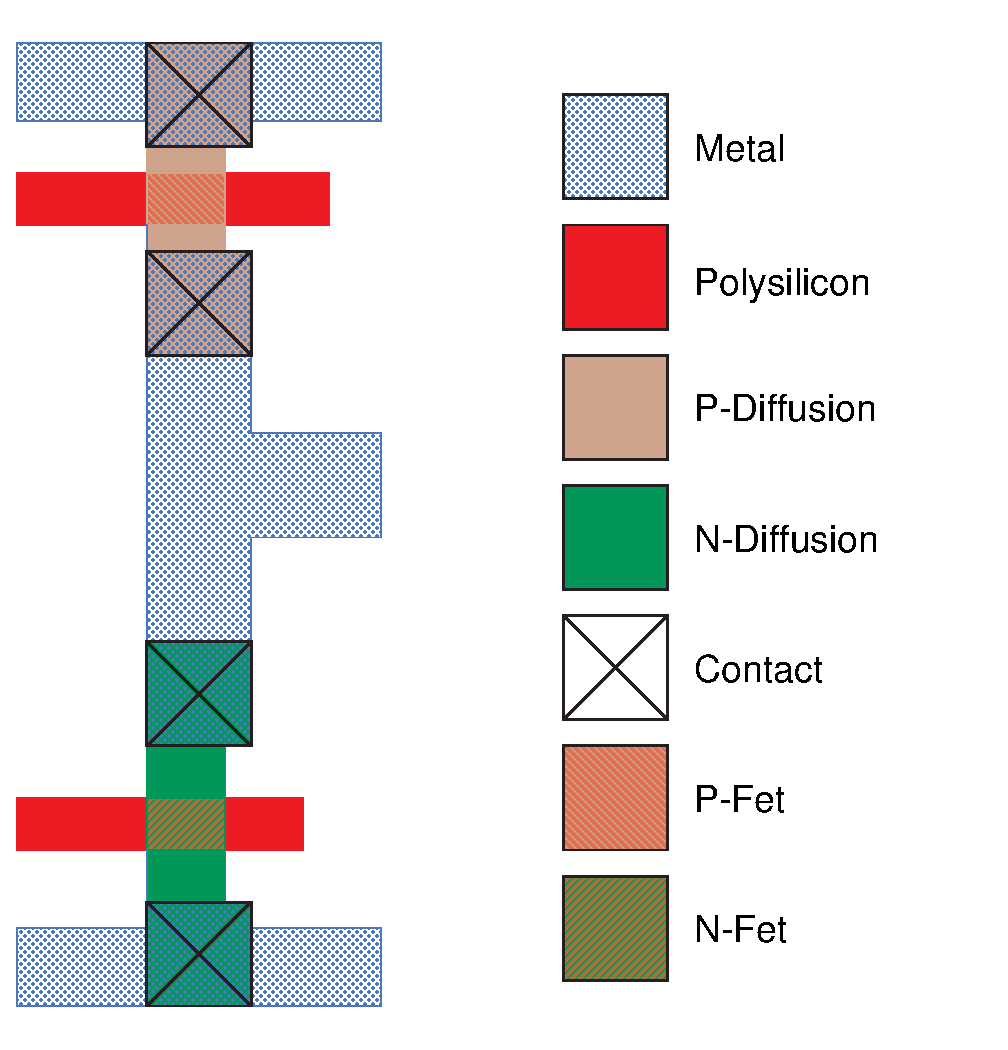
\epsfig{file=../psfigures/tut2.1.ps, height=4.0in}
   \end{minipage}
   \caption {An example of how the logs are used.  The figure on
	the left shows actual mask layers for an CMOS inverter
	cell, and the figure on the right shows the layers used
	to represent the cell in Magic.}
   \label{layers1}
   \end{center}
\end{figure}

An advantage of the logs used in Magic is
that they simplify the design rules.  Most of the formation
rules (e.g. contact structure) go away, since Magic automatically
generates correctly-formed structures when it writes CIF.
All that are left are minimum size and spacing rules, and
Magic's abstract layers result in fewer of these than there
would be otherwise.  This helps to make Magic's built-in
design rule checker very fast (see ``Magic Tutorial  \#6:
Design Rule Checking''), and is one of the reasons
plowing is possible.

\end{document}
